\let\negmedspace\undefined
\let\negthickspace\undefined
\documentclass[journal]{IEEEtran}
\usepackage[a5paper, margin=10mm, onecolumn]{geometry}
%\usepackage{lmodern} % Ensure lmodern is loaded for pdflatex
\usepackage{tfrupee} % Include tfrupee package

\setlength{\headheight}{1cm} % Set the height of the header box
\setlength{\headsep}{0mm}     % Set the distance between the header box and the top of the text
\usepackage{multicol}
\usepackage{gvv-book}
\usepackage{gvv}
\usepackage{cite}
\usepackage{amsmath,amssymb,amsfonts,amsthm}
\usepackage{algorithmic}
\usepackage{graphicx}
\usepackage{textcomp}
\usepackage{xcolor}
\usepackage{txfonts}
\usepackage{listings}
\usepackage{enumitem}
\usepackage{mathtools}
\usepackage{gensymb}
\usepackage{comment}
\usepackage[breaklinks=true]{hyperref}
\usepackage{tkz-euclide} 
\usepackage{pgfplots}
\pgfplotsset{compat=1.18}
\usepackage{listings}
% \usepackage{gvv}                                        
\def\inputGnumericTable{}                                 
\usepackage[latin1]{inputenc}                                
\usepackage{color}                                            
\usepackage{array}                                            
\usepackage{longtable}                                       
\usepackage{calc}                                             
\usepackage{multirow}                                         
\usepackage{hhline}                                           
\usepackage{ifthen}                                           
\usepackage{lscape}
\usepackage{tikz}
% Marks the beginning of the document
\begin{document}
\bibliographystyle{IEEEtran}
\vspace{3cm}

\title{9-5-8}
\author{EE24BTECH11060 - sruthi bijili}
\maketitle
%\newpage
\bigskip

\renewcommand{\thefigure}{\theenumi}
\renewcommand{\thetable}{\theenumi}
\textbf{Question}:\\
Solve the following differential equation $x\frac{dy}{dx}$ = $y-x\sin{\frac{y}{x}}$\\

\textbf{Theoretical solution}:\\
\text{given equation}\\
\begin{align}
    x\frac{dy}{dx}=y-x\sin{\frac{y}{x}}\\
    \implies \frac{dy}{dx}=\frac{y}{x}-\sin{\frac{y}{x}}\\
\end{align}
\text{let y=vx}
\text{by doing partial differentiation with respect to  x}\\
\begin{align}
    \frac{dy}{dx}=v+x\frac{dv}{dx}
\end{align}
substitute in given equation
\begin{align}
    v+x\frac{dv}{dx}=v-\sin{v}\\
    x\frac{dv}{dx}=-\sin{v}\\
    \frac{dv}{\sin{v}}=-\frac{1}{x}dx\\
\end{align}
integrating on both sides
\begin{align}
    \int{\csc{v}}dv=-\int{\frac{1}{x}}dx\\
    \log{\tan{\frac{v}{2}}}=-\log{x}+\log{k}\\
    \log{\tan{\frac{v}{2}}}=\log{\frac{k}{x}}\\
\end{align}
\text{let k be any constant}
\begin{align}
    \tan{\frac{v}{2}}=\frac{1}{x}\\
    \tan{\frac{y}{2x}}=\frac{1}{x}\\
    \frac{y}{2x}=tan^{-1}{\frac{1}{x}}\\
    y=2x\tan^{-1}{\frac{1}{x}}
\end{align}
\textbf{method of finite differences}\\
The derivative of f(x) can be written as 
\begin{align}
    \frac{df}{dx}=\frac{f(x+h)-f(x)}{h}\\
    \implies f(x+h)=f(x)+h\cdot\frac{dy}{dx}
\end{align}
from the above question 
\begin{align}
    \frac{dy}{dx}=\frac{y}{x}-\sin{\frac{y}{x}}\\
    \implies y(x+h)=y(x)+h\cdot \frac{y}{x}-\sin{\frac{y}{x}}
\end{align}
for $x \in \sbrak{x_{0},x_{n}}$ divide into equal parts by difference h\\
Let $x_{1}$=$x_{0}+h$ then 
\begin{align}
    y_{1}=y_{0}+h\cdot \frac{y_{0}}{x_{0}}-\sin{\frac{y_{0}}{x_{0}}}
\end{align}
 To obtain the graph repeat the process until sufficient points to plot the graph and the general equation will be 
\begin{align}
    x_{n+1}=x_{n}+h\\
    y_{n+1}=y_{n}+h\cdot \frac{y_{n}}{x_{n}}-\sin{\frac{y_{n}}{x_{n}}}
\end{align}
The curve generalised using the method of finite differences for the given question taking $x_{0}=1$,$y_{0}=1$, $h=0.1$ and running iterations for 100 times
\begin{figure}[h!]
   \centering
   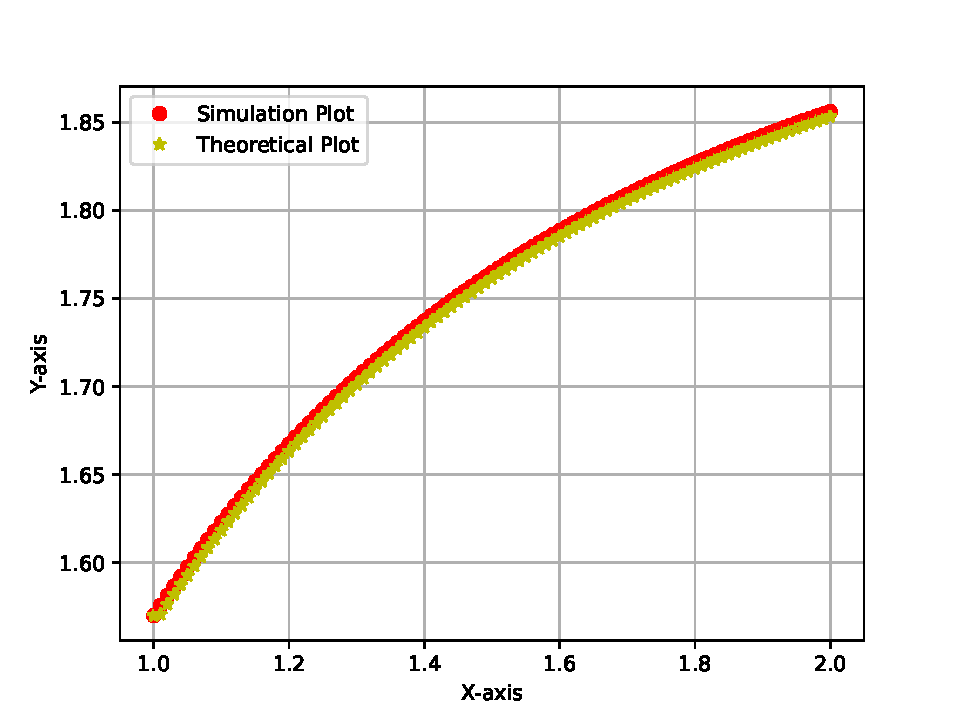
\includegraphics[width=0.7\columnwidth]{figs/fig.pdf}
\end{figure}

\end{document}

